% !TEX root = template.tex

\begin{table*}[t]
	\begin{center}
		\begin{tabular}{ p{7cm}p{2cm}p{2cm}p{2cm}p{2cm} } 
			\hline
			Method & Accuracy & Precision & Recall & F1-Score \\ 
			\hline
			CNN + No centering & 77.0 & 78.0 & 75.8 & 76.8 \\ 
			CNN + No centering + Manual F. & 75.6 & 76.8 & 73.9 & 75.3 \\
			CNN + Centering + Manual F. & 86.2 & 86.9 & 70.2 & 77.6 \\ 
			\textbf{CNN + Centering + Encoder F.} & \textbf{89.2} & \textbf{88.9} &  \textbf{86.1} & \textbf{86.1} \\ 
			\hline
		\end{tabular}
		\caption{\label{tab:model-performance} UCI classification results with different featueres CNN augumentation and data preprocessing. The test are made with our CNN with OIT, Data centering, 196 (1x16) filters, max-pool (1x4), 64 fully conected, l2-regularization of 5e-5 and Adam learning rate of 2e-5.}
	\end{center}
\end{table*}

\section{Results}
\label{sec:results}
In this section we will present how we selected the appropriate hyper parameters for the final proposed architecture presented in Sec. \ref{sec:learning_framework}. Then we will see how some of the preprocessing blocks and encoder and manual extracted features influence performance onto the Heterogenity Dataset. An in the last part we will test the proposed archittecture with OIT in our collected dataset.  

\subsection{Heterogenity Dataset (HD)}

In this section we evaluate performance between previous work and different model architectures and the influences of some of the pre-processing techniques applied. Similar to what was done in \cite{ignatov2018real} we caried out from the HD dataset some representative users to test the model and then use the remaining ones to train the model. In this case we selected user a and b since we found that these two users are very representative of all the remaining user, in fact models tend to be less precise with user a and more accurate with user b and this mainly depends with the style that user usually performs the type of activity considered. In this way we are able to compare results with other works that usually tend to evaluate performances on unseen user. 

In this training and test set settings, we evaluate the best hyperparameters for the proposed architecture model excluding OIT preprocessing block, since this dataset was collected with a fixed orientation. The rest of pre-processing techinque are enabled, if not specified.\\ 

\textbf{Autoencoder}\\
TODO Parlare dei risultati ottenuti da luca con un semplice autoencoder sia K-NN classifier che con FFNN alla fine. Un concetto alla volta!

\textbf{CNN Network}

We fist test how number of convolutional filters and number of dense neurons in the FC2 layer will influence classification performances. The results obtained are presented in Tab. \ref{tab:model-selection}. Wee decided to choose 196 convolutional filters and 64 dense neurons thanks to its balance between accuracy and F1-Score performance, obtaining 88.9\% accuracy score and  81.6\%. To compare our result with that obtained in the original work \cite{blunck2013heterogeneity}, we decided to perform their \textit{Leave-one-user-out cross validation} evaluation, consisting of test the model with data from one user, and train with data from all the others in a cross validation fashion and then averaging the metrics obtained. In this evaluation setting we obtained an average F1-score of 85.8\%, beating their best model result of nearly 10\% more of F1-Score metrics. This prove also that using users a and b to do our evaluation is a good compromise of the real \textit{Leave-one-user-out cross validation} evaluation performances, since we obtain nearly the same results (90.2\% instead of 88.9\% in accuracy and 85.8\% instead of 81.6\%). TODO scrivere nelle conslusione che in questo settings abbiamo notato un bel po di varianza tra utenti.

\begin{table}[h]
	\begin{center}
		\begin{tabular}{ p{1.8cm}p{1.7cm}p{1.7cm}p{1.7cm} } 
			\hline
			CNN Filters & Dense Neurons & Accuracy & F1-Score \\ 
			\hline
			196 & 1024 & 84.6 & 75.3 \\
			196 & 512 & 86.1 & 75.7 \\ 
			\textbf{196} & \textbf{64} & \textbf{88.9} & \textbf{81.6} \\ 
			96 & 1024 & 82.8 & 69.9 \\
			96 & 512 & 84.4 & 73.7 \\ 
			96 & 64 & 89.0 & 73.0 \\  
			48 & 1024 & 80.0 & 79.4 \\
			48 & 512 & 83.7 & 74.9 \\ 
			48 & 64 & 84.0 & 72.3 \\
			\hline
		\end{tabular}
		\caption{\label{tab:model-selection} UCI classification results with data centering and manual features augmented CNN}
	\end{center}
\end{table}


To better appreciate how our pre-processing block affects model overall performance, we also try to disable or enable some of these blocks. In Tab. \ref{tab:model-performance} we report our obtained results experiments. We see that augmenting the CNN with manual extracted feature when data are not centered, lead to no significant change in performances, instead when also enable data centering pre-processing with manual features augmented CNN the model obtain nearly 10\% more in accuracy and precision metrics. This prove the benefits of data centering stated previously. However we were not able to get the same performances obtained in \cite{ignatov2018real}, where the authors obtained in the same exact setting an accuracy of 97.6\%. These empirically confirm that performances of state-of-the-art models trained with one type of sensors are worse when dealing with smartphone sensor heterogeneity. Moving on, augmenting the CNN with encoder feature lead the model to better performances, meaning that encoder feature are more robust that manual feature, as explained previously. A confusion matrix in this latter setting is reported in Fig. \ref{fig:cnn-confusion-matrix} where we could see that the model perform nicely overall in all the considered activities, with some difficulties in distinguishing between stationary activities, stand and sit, and walk activity with stairs since that activities are very similar sensor signals foot-prints.

\begin{figure}[h]
	\centering
	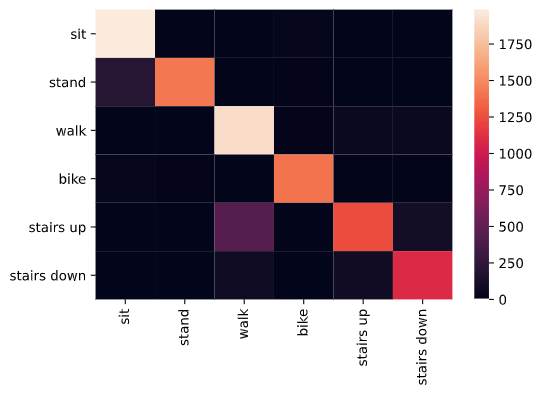
\includegraphics[width=0.5\textwidth]{images/confusion_matrix.png}
	\caption{CNN confusion matrix}
	\label{fig:cnn-confusion-matrix}
\end{figure}


\subsection{Oriented Dataset (OD)}




\begin{table}[t]
	\begin{center}
		\begin{tabular}{ p{1.8cm}p{1.2cm}p{1.2cm}p{0.9cm}p{1.4cm}} 
			\hline
			Positions & Accuracy & Precision & Recall & F1-Score \\ 
			\hline
			Pouch \\(L,R,T,B) & 85.3 & 92.0 & 73.8 & 81.9 \\ 
			\hline
			Hand, \\ Pocket U\&D & 70.5 & 79.5 & 63.0 & 70.2 \\
			\hline
			All & 78.0 & 84.0 & 69.0 & 75.7 \\
			\hline
		\end{tabular}
		\caption{\label{tab:model-performance} Classification comparisons onto Oriented Dataset between only certain selected smartphone positions using our proposed architecture augmented with encoder features. We apply OIT, Data centering, 196 (1x16) filters, max-pool (1x4), 64 fully conected, l2-regularization of $5e^{-5}$ and Adam with learning rate of $2e^{-5}$. }
	\end{center}
\end{table}


